\documentclass[tikz,border=2mm]{standalone}
\usepackage{tikz}
\usetikzlibrary{arrows.meta,positioning,calc,fit,shapes.geometric,backgrounds}
\usepackage{booktabs}
\usepackage{colortbl}
\usepackage{enumitem}
\usepackage{lmodern}

\begin{document}
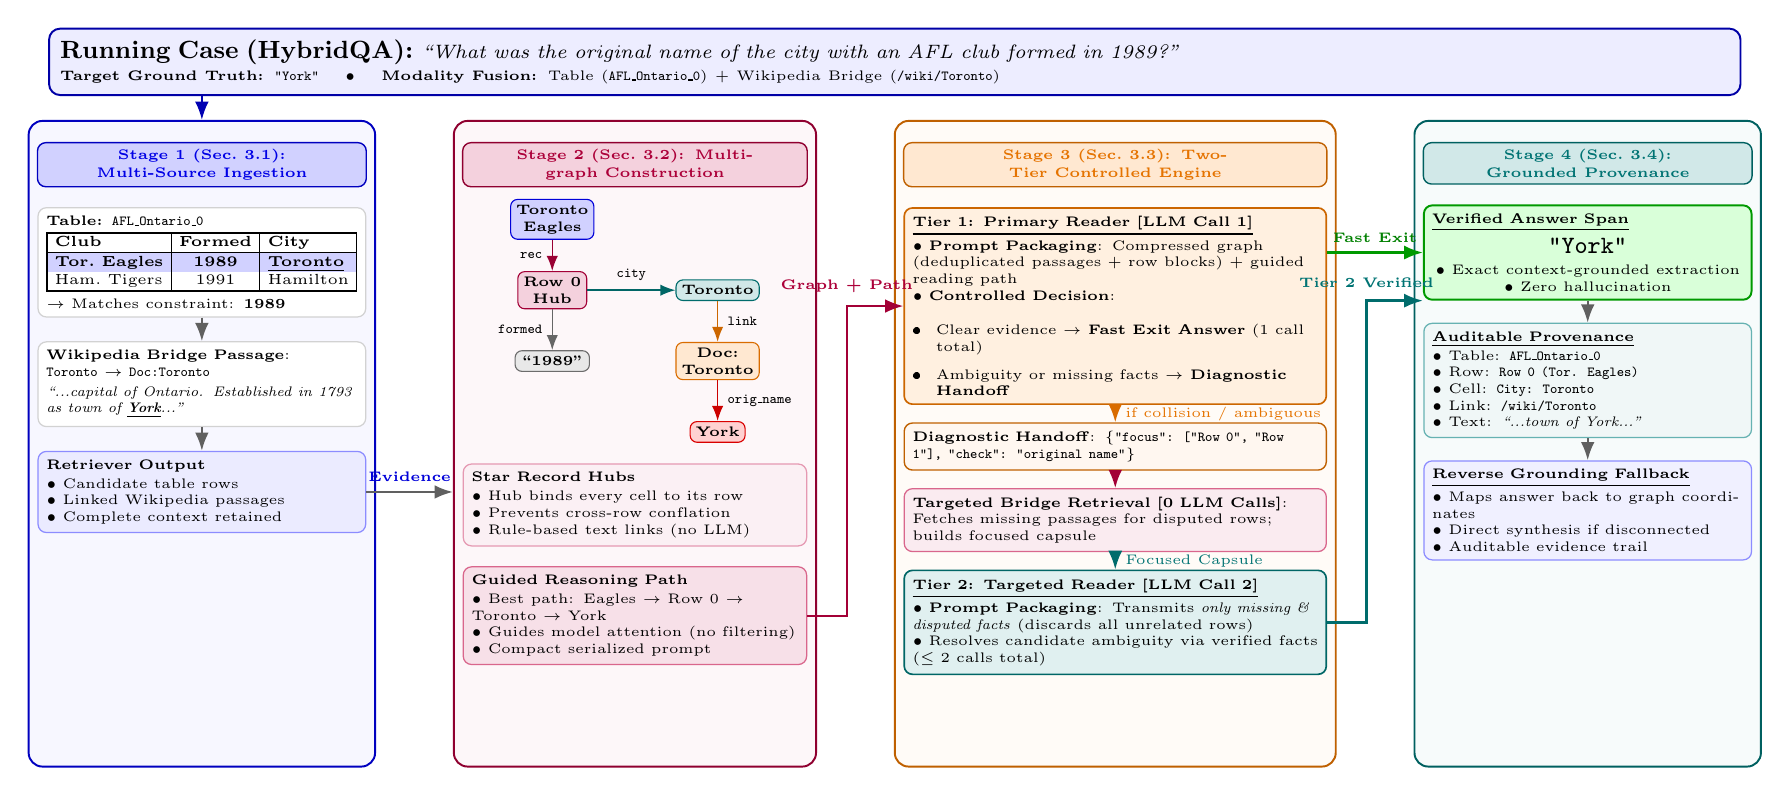
\begin{tikzpicture}[
  >=Latex,
  font=\scriptsize,
  panel/.style={draw=#1!75!black, fill=#1!3, rounded corners=5pt, line width=0.7pt},
  titlebar/.style={fill=#1!18, draw=#1!75!black, line width=0.5pt, rounded corners=3pt, font=\bfseries\fontsize{5.2pt}{6.2pt}\selectfont, text=#1!90!black, align=center, inner sep=2.5pt, minimum height=4.2mm},
  subcard/.style={draw=gray!35, fill=white, rounded corners=3pt, align=left, inner sep=3pt, font=\tiny, line width=0.45pt},
  llmcard/.style={draw=#1!80!black, fill=#1!12, rounded corners=3pt, align=left, inner sep=3pt, font=\tiny, line width=0.6pt},
  flow/.style={->, line width=0.8pt, draw=gray!75!black},
  flow_teal/.style={->, line width=0.85pt, draw=teal!85!black},
  flow_green/.style={->, line width=0.85pt, draw=green!60!black},
  flow_orange/.style={->, line width=0.8pt, draw=orange!85!black},
  flow_purple/.style={->, line width=0.8pt, draw=purple!85!black},
  knode/.style={draw=#1!85!black, fill=#1!18, rounded corners=2.5pt, inner sep=2pt, font=\tiny\bfseries, align=center},
  kedge/.style={->, line width=0.55pt, draw=#1!80!black, font=\tiny}
]

% ========================================================
% TOP BANNER: RUNNING USE CASE QUESTION
% Total width: 22.0cm, Center: 11.00
% ========================================================
\node[draw=blue!65!black, fill=blue!7, rounded corners=4pt, line width=0.7pt, text width=21.2cm, inner sep=4pt, align=left] (q_box) at (11.00, 4.35) {
  \textbf{\small Running Case (HybridQA):} \textit{``What was the original name of the city with an AFL club formed in 1989?''} \\
  \tiny \textbf{Target Ground Truth:} \texttt{"York"} \quad $\bullet$ \quad \textbf{Modality Fusion:} Table (\texttt{AFL\_Ontario\_0}) $+$ Wikipedia Bridge (\texttt{/wiki/Toronto})
};

% ========================================================
% STAGE 1: MULTI-SOURCE EVIDENCE INGESTION (Sec. 3.1)
% Panel: [0.0, 4.4], Center: 2.20, Width: 4.4
% ========================================================
\node[panel=blue, minimum width=4.4cm, minimum height=8.2cm] (panel1) at (2.20, -0.5) {};
\node[titlebar=blue, text width=4.0cm, anchor=north] (t1) at ([yshift=-2.8mm]panel1.north) {Stage 1 (Sec.~3.1): Multi-Source Ingestion};

\node[subcard, text width=3.95cm, anchor=north] (table_box) at ([yshift=-2.5mm]t1.south) {
  {\fontsize{5pt}{6pt}\selectfont
  \textbf{Table: \texttt{AFL\_Ontario\_0}} \\[0.5mm]
  \resizebox{\linewidth}{!}{%
  \renewcommand{\arraystretch}{1.05}%
  \setlength{\tabcolsep}{2.5pt}%
  \begin{tabular}{|l|c|l|}
    \hline
    \textbf{Club} & \textbf{Formed} & \textbf{City} \\
    \hline
    \rowcolor{blue!18} \textbf{Tor.\ Eagles} & \textbf{1989} & \textbf{\underline{Toronto}} \\
    Ham.\ Tigers & 1991 & Hamilton \\
    \hline
  \end{tabular}%
  }\\[0.6mm]
  $\rightarrow$ Matches constraint: \textbf{1989}
  \par}
};

\node[subcard, text width=3.95cm, anchor=north] (link_box) at ([yshift=-3mm]table_box.south) {
  {\fontsize{5pt}{6pt}\selectfont
  \textbf{Wikipedia Bridge Passage}: \\
  \texttt{Toronto} $\rightarrow$ \texttt{Doc:Toronto} \\[0.4mm]
  \textit{``...capital of Ontario. Established in 1793 as town of \textbf{\underline{York}}...''}
  \par}
};

\node[subcard, text width=3.95cm, fill=blue!8, draw=blue!45, anchor=north] (retr_summary) at ([yshift=-3mm]link_box.south) {
  {\fontsize{5pt}{6pt}\selectfont
  \textbf{Retriever Output} \\[0.3mm]
  $\bullet$ Candidate table rows \\
  $\bullet$ Linked Wikipedia passages \\
  $\bullet$ Complete context retained
  \par}
};

\draw[flow] (table_box.south) -- (link_box.north);
\draw[flow] (link_box.south) -- (retr_summary.north);

% ========================================================
% STAGE 2: SCHEMA-PRESERVING MULTIGRAPH (Sec. 3.2)
% Panel: [5.4, 10.0], Center: 7.70, Width: 4.6
% ========================================================
\node[panel=purple, minimum width=4.6cm, minimum height=8.2cm] (panel2) at (7.70, -0.5) {};
\node[titlebar=purple, text width=4.2cm, anchor=north] (t2) at ([yshift=-2.8mm]panel2.north) {Stage 2 (Sec.~3.2): Multigraph Construction};

% Graph nodes
\node[knode=blue] (ent_club) at (6.65, 2.35) {Toronto\\Eagles};
\node[knode=purple] (rec_node) at (6.65, 1.45) {Row 0\\Hub};
\node[knode=teal] (ent_city) at (8.75, 1.45) {Toronto};
\node[knode=gray] (lit_year) at (6.65, 0.55) {``1989''};
\node[knode=orange] (doc_node) at (8.75, 0.55) {Doc:\\Toronto};
\node[knode=red] (ans_node_g) at (8.75, -0.35) {York};

% Graph edges
\draw[kedge=purple] (ent_club) -- node[left, font=\tiny] {\texttt{rec}} (rec_node);
\draw[kedge=teal] (rec_node) -- node[above, font=\tiny] {\texttt{city}} (ent_city);
\draw[kedge=gray] (rec_node) -- node[left, font=\tiny] {\texttt{formed}} (lit_year);
\draw[kedge=orange] (ent_city) -- node[right, font=\tiny] {\texttt{link}} (doc_node);
\draw[kedge=red] (doc_node) -- node[right, font=\tiny] {\texttt{orig\_name}} (ans_node_g);

\node[subcard, text width=4.15cm, fill=purple!6, draw=purple!40, anchor=north] (centroid_box) at (7.70, -0.75) {
  {\fontsize{5pt}{6pt}\selectfont
  \textbf{Star Record Hubs} \\[0.3mm]
  $\bullet$ Hub binds every cell to its row \\
  $\bullet$ Prevents cross-row conflation \\
  $\bullet$ Rule-based text links (no LLM)
  \par}
};

\node[subcard, text width=4.15cm, fill=purple!12, draw=purple!60, anchor=north] (path_box) at ([yshift=-2.5mm]centroid_box.south) {
  {\fontsize{5pt}{6pt}\selectfont
  \textbf{Guided Reasoning Path} \\[0.3mm]
  $\bullet$ Best path: Eagles $\to$ Row 0 $\to$ Toronto $\to$ York \\
  $\bullet$ Guides model attention (no filtering) \\
  $\bullet$ Compact serialized prompt
  \par}
};

% ========================================================
% STAGE 3: TWO-TIER CONTROLLED REASONING ENGINE (Sec. 3.3)
% Panel: [11.0, 16.6], Center: 13.80, Width: 5.6
% ========================================================
\node[panel=orange, minimum width=5.6cm, minimum height=8.2cm] (panel3) at (13.80, -0.5) {};
\node[titlebar=orange, text width=5.2cm, anchor=north] (t3) at ([yshift=-2.8mm]panel3.north) {Stage 3 (Sec.~3.3): Two-Tier Controlled Engine};

% Tier 1 LLM Card
\node[llmcard=orange, text width=5.15cm, anchor=north] (l1_box) at ([yshift=-2.5mm]t3.south) {
  {\fontsize{5pt}{6pt}\selectfont
  \textbf{\underline{Tier 1: Primary Reader [LLM Call 1]}} \\[0.3mm]
  $\bullet$ \textbf{Prompt Packaging}: Compressed graph (deduplicated passages $+$ row blocks) $+$ guided reading path \\
  $\bullet$ \textbf{Controlled Decision}:
  \vspace{-0.5mm}
  \begin{itemize}[leftmargin=3mm]
    \setlength{\itemsep}{0pt}
    \item Clear evidence $\rightarrow$ \textbf{Fast Exit Answer} (1 call total)
    \item Ambiguity or missing facts $\rightarrow$ \textbf{Diagnostic Handoff}
  \end{itemize}
  \par}
};

% Diagnostic Packet Box
\node[subcard, text width=5.15cm, fill=orange!6, draw=orange!75!black, line width=0.5pt, anchor=north] (handoff_box) at ([yshift=-2.2mm]l1_box.south) {
  {\fontsize{5pt}{6pt}\selectfont
  \textbf{Diagnostic Handoff}: \texttt{\{"focus": ["Row 0", "Row 1"], "check": "original name"\}}
  \par}
};

% Targeted Bridge Re-retrieval
\node[subcard, text width=5.15cm, fill=purple!8, draw=purple!60, anchor=north] (ret_box) at ([yshift=-2.2mm]handoff_box.south) {
  {\fontsize{5pt}{6pt}\selectfont
  \textbf{Targeted Bridge Retrieval [0 LLM Calls]}: \\
  Fetches missing passages for disputed rows; builds focused capsule
  \par}
};

% Tier 2 LLM Card
\node[llmcard=teal, text width=5.15cm, anchor=north] (l2_box) at ([yshift=-2.2mm]ret_box.south) {
  {\fontsize{5pt}{6pt}\selectfont
  \textbf{\underline{Tier 2: Targeted Reader [LLM Call 2]}} \\[0.3mm]
  $\bullet$ \textbf{Prompt Packaging}: Transmits \emph{only missing \& disputed facts} (discards all unrelated rows) \\
  $\bullet$ Resolves candidate ambiguity via verified facts ($\le 2$ calls total)
  \par}
};

\draw[flow_orange] (l1_box.south) -- node[right, font=\tiny, text=orange!90!black] {if collision / ambiguous} (handoff_box.north);
\draw[flow_purple] (handoff_box.south) -- (ret_box.north);
\draw[flow_teal] (ret_box.south) -- node[right, font=\tiny, text=teal!90!black] {Focused Capsule} (l2_box.north);

% ========================================================
% STAGE 4: GROUNDED GENERATION & PROVENANCE AUDIT (Sec. 3.4)
% Panel: [17.6, 22.0], Center: 19.80, Width: 4.4
% ========================================================
\node[panel=teal, minimum width=4.4cm, minimum height=8.2cm] (panel4) at (19.80, -0.5) {};
\node[titlebar=teal, text width=4.0cm, anchor=north] (t4) at ([yshift=-2.8mm]panel4.north) {Stage 4 (Sec.~3.4): Grounded Provenance};

% Answer box aligned with l1_box center vertically!
\node[subcard, text width=3.95cm, fill=green!15, draw=green!60!black, line width=0.7pt, anchor=north] (ans_box) at ([yshift=-2.5mm]t4.south) {
  {\fontsize{5pt}{6pt}\selectfont
  \textbf{\underline{Verified Answer Span}} \\[0.5mm]
  \centering{\textbf{\small \texttt{"York"}}}\\[0.6mm]
  $\bullet$ Exact context-grounded extraction \\
  $\bullet$ Zero hallucination
  \par}
};

\node[subcard, text width=3.95cm, fill=teal!6, draw=teal!60, anchor=north] (prov_box) at ([yshift=-2.8mm]ans_box.south) {
  {\fontsize{5pt}{6pt}\selectfont
  \textbf{\underline{Auditable Provenance}} \\[0.3mm]
  $\bullet$ Table: \texttt{AFL\_Ontario\_0} \\
  $\bullet$ Row: \texttt{Row 0 (Tor. Eagles)} \\
  $\bullet$ Cell: \texttt{City: Toronto} \\
  $\bullet$ Link: \texttt{/wiki/Toronto} \\
  $\bullet$ Text: \textit{``...town of York...''}
  \par}
};

\node[subcard, text width=3.95cm, fill=blue!6, draw=blue!45, anchor=north] (rev_box) at ([yshift=-2.8mm]prov_box.south) {
  {\fontsize{5pt}{6pt}\selectfont
  \textbf{\underline{Reverse Grounding Fallback}} \\[0.3mm]
  $\bullet$ Maps answer back to graph coordinates \\
  $\bullet$ Direct synthesis if disconnected \\
  $\bullet$ Auditable evidence trail
  \par}
};

\draw[flow] (ans_box.south) -- (prov_box.north);
\draw[flow] (prov_box.south) -- (rev_box.north);

% ========================================================
% INTER-STAGE CONNECTORS (Orthogonal & Neat)
% ========================================================
% Top question to Stage 1
\draw[flow, draw=blue!70!black] (q_box.south -| panel1.north) -- (panel1.north);

% Stage 1 -> Stage 2 (Clean horizontal line in 1.0cm gap)
\draw[flow] (retr_summary.east) -- node[above, font=\tiny\bfseries, text=blue!85!black] {Evidence} (panel2.west |- retr_summary.east);

% Stage 2 -> Stage 3 (Orthogonal neat step into Tier 1 reader in 1.0cm gap)
\path (path_box.east) -- ++(0.50, 0) coordinate (p_turn);
\draw[flow, draw=purple!85!black] (path_box.east) -- (p_turn) -- (p_turn |- l1_box.west) node[above=1pt, font=\tiny\bfseries, text=purple!90!black] {Graph + Path} -- (l1_box.west);

% Stage 3 -> Stage 4: Branch 1: Tier 1 Fast Exit (Pure horizontal line in 1.0cm gap!)
\draw[flow_green] (l1_box.east |- ans_box.center) -- node[above, font=\tiny\bfseries, text=green!50!black] {Fast Exit} (ans_box.west);

% Stage 3 -> Stage 4: Branch 2: Tier 2 Verified Exit (Orthogonal right-angle step into ans_box!)
\path (l2_box.east) -- ++(0.50, 0) coordinate (t_turn);
\draw[flow_teal] (l2_box.east) -- (t_turn) -- (t_turn |- ans_box.south west) node[above=1pt, font=\tiny\bfseries, text=teal!90!black] {Tier 2 Verified} -- (ans_box.south west);


\path (panel1.south); \pgfgetlastxy{\px}{\py}; \typeout{PANEL1_S: \py}
\path (retr_summary.south); \pgfgetlastxy{\px}{\py}; \typeout{RETR_S: \py}
\path (panel2.south); \pgfgetlastxy{\px}{\py}; \typeout{PANEL2_S: \py}
\path (path_box.south); \pgfgetlastxy{\px}{\py}; \typeout{PATH_S: \py}
\path (panel3.south); \pgfgetlastxy{\px}{\py}; \typeout{PANEL3_S: \py}
\path (l2_box.south); \pgfgetlastxy{\px}{\py}; \typeout{L2_S: \py}
\path (panel4.south); \pgfgetlastxy{\px}{\py}; \typeout{PANEL4_S: \py}
\path (rev_box.south); \pgfgetlastxy{\px}{\py}; \typeout{REV_S: \py}
\end{tikzpicture}
\end{document}